% fig_arch.tex — skema Mamba-YOLO-T, SS2D tetap vs DeformSS2D (k3_replace).
% Diverifikasi terhadap: DeMamba-YOLO-T.yaml (lapis 1,3,5[x3],7 backbone; 11,14,17,20 neck; skala T: 9 -> 3 blok),
% deform_ss2d.py (cross_scan_axial: row, col, row-rev, col-rev; k3_replace: row, row-rev, deformable;
% DeformableScan: tanh*1/(H-1) -> <=0.5 px; posisi = ref + tanh(dp) -> argsort; reverse = permutasi balik).
\documentclass[border=1pt]{standalone}
\usepackage{mathptmx}
\usepackage{tikz}
\usetikzlibrary{arrows.meta,positioning,fit,calc,backgrounds}
\definecolor{dblue}{HTML}{2A78D6}
\definecolor{dbluel}{HTML}{DCE9F8}
\definecolor{gry}{HTML}{8D8C88}
\definecolor{gryl}{HTML}{F0EFEC}
\definecolor{ink}{HTML}{0B0B0B}
\definecolor{muted}{HTML}{52514E}
\newcommand{\grid}[2]{% #1 = x, #2 = y (top-left)
  \foreach \i in {0,1,2} \foreach \j in {0,1,2} \fill[gry] ($(#1,#2)+(0.3*\i,-0.3*\j)$) circle (0.75pt);}
\begin{document}
\footnotesize
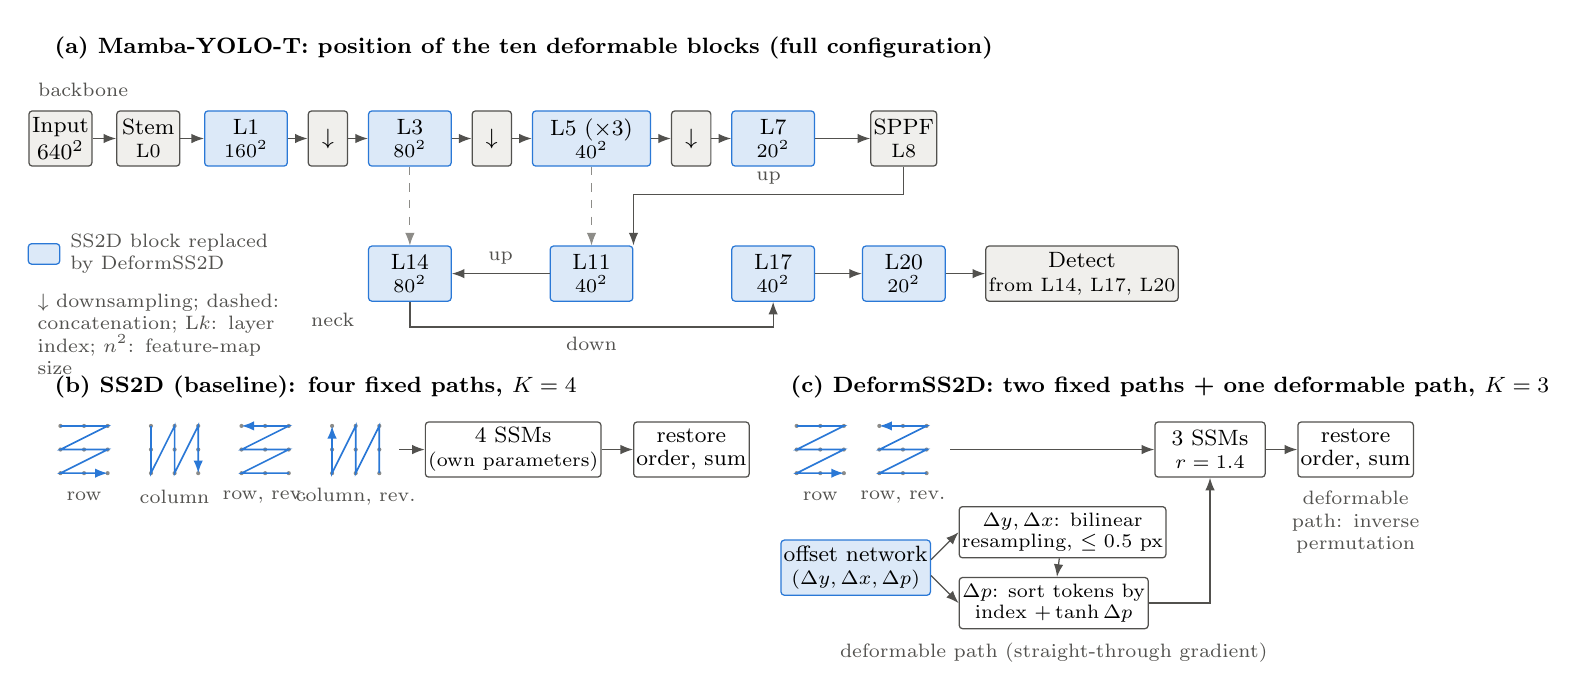
\begin{tikzpicture}[
  >={Latex[length=1.6mm,width=1.2mm]}, font=\footnotesize, line width=0.45pt, draw=muted,
  blk/.style={draw=muted, rounded corners=1.2pt, minimum height=7mm, minimum width=10.5mm, align=center, inner sep=1pt, fill=white},
  dfb/.style={blk, fill=dbluel, draw=dblue},
  aux/.style={blk, minimum width=8mm, fill=gryl},
  lab/.style={font=\scriptsize, text=muted, align=center},
  flow/.style={->, draw=muted},
  lat/.style={->, draw=gry, dashed, line width=0.35pt},
  ttl/.style={font=\footnotesize\bfseries, anchor=west}
]
% ======================= (a) Mamba-YOLO-T =======================
\node[ttl] at (-0.2, 1.15) {(a) Mamba-YOLO-T: position of the ten deformable blocks (full configuration)};
\node[aux] (in) at (0,0) {Input\\$640^2$};
\node[aux, right=3mm of in] (stem) {Stem\\[-1pt]{\scriptsize L0}};
\node[dfb, right=3mm of stem] (l1) {L1\\[-1pt]{\scriptsize $160^2$}};
\node[aux, right=2.5mm of l1, minimum width=5mm] (d2) {$\downarrow$};
\node[dfb, right=2.5mm of d2] (l3) {L3\\[-1pt]{\scriptsize $80^2$}};
\node[aux, right=2.5mm of l3, minimum width=5mm] (d4) {$\downarrow$};
\node[dfb, right=2.5mm of d4, minimum width=15mm] (l5) {L5 ($\times$3)\\[-1pt]{\scriptsize $40^2$}};
\node[aux, right=2.5mm of l5, minimum width=5mm] (d6) {$\downarrow$};
\node[dfb, right=2.5mm of d6] (l7) {L7\\[-1pt]{\scriptsize $20^2$}};
\node[aux, right=7mm of l7] (sppf) {SPPF\\[-1pt]{\scriptsize L8}};
\foreach \a/\b in {in/stem, stem/l1, l1/d2, d2/l3, l3/d4, d4/l5, l5/d6, d6/l7, l7/sppf} \draw[flow] (\a) -- (\b);
% neck (PAFPN): L11 (P4) <- L14 (P3) -> L17 (P4) -> L20 (P5)
\node[dfb, below=10mm of l5] (l11) {L11\\[-1pt]{\scriptsize $40^2$}};
\node[dfb, below=10mm of l3] (l14) {L14\\[-1pt]{\scriptsize $80^2$}};
\node[dfb, below=10mm of l7] (l17) {L17\\[-1pt]{\scriptsize $40^2$}};
\node[dfb, below=10mm of sppf] (l20) {L20\\[-1pt]{\scriptsize $20^2$}};
\node[aux, right=5mm of l20, minimum width=16mm] (det) {Detect\\[-1pt]{\scriptsize from L14, L17, L20}};
\draw[flow] (sppf.south) -- ++(0,-0.35) -| node[lab, above, pos=0.25]{up} (l11.north east);
\draw[flow] (l11) -- node[lab, above]{up} (l14);
\draw[flow] (l14.south) -- ++(0,-0.32) -| node[lab, below, pos=0.25]{down} (l17.south);
\draw[flow] (l17) -- (l20);
\draw[flow] (l20) -- (det);
\draw[lat] (l5) -- (l11); \draw[lat] (l3) -- (l14);
\node[lab, anchor=south west] at ($(in.north west)+(0,0.05)$) {backbone};
\node[lab, anchor=north east] at ($(l14.south west)+(-0.05,-0.02)$) {neck};
% legend for (a)
\node[dfb, minimum width=4mm, minimum height=2.6mm] (lg1) at ($(in.west |- l14)+(0.2,0.25)$) {};
\node[lab, anchor=west, align=left] at (lg1.east) {SS2D block replaced\\by DeformSS2D};
\node[lab, anchor=north west, text width=33mm, align=left] at ($(lg1.south west)+(0,-0.25)$) {$\downarrow$ downsampling; dashed: concatenation; L$k$: layer index; $n^2$: feature-map size};

% ======================= (b) fixed SS2D =======================
\begin{scope}[shift={(0,-4.1)}]
\node[ttl] at (-0.2, 0.95) {(b) SS2D (baseline): four fixed paths, $K=4$};
% row-major
\grid{0}{0.45}
\draw[dblue, ->, line width=0.6pt] (0,0.45)--(0.6,0.45) -- (0,0.15) -- (0.6,0.15) -- (0,-0.15) -- (0.6,-0.15);
\node[lab] at (0.3,-0.45) {row};
\grid{1.15}{0.45}
\draw[dblue, ->, line width=0.6pt] (1.15,0.45)--(1.15,-0.15) -- (1.45,0.45) -- (1.45,-0.15) -- (1.75,0.45) -- (1.75,-0.15);
\node[lab] at (1.45,-0.45) {column};
\grid{2.3}{0.45}
\draw[dblue, ->, line width=0.6pt] (2.9,-0.15)--(2.3,-0.15) -- (2.9,0.15) -- (2.3,0.15) -- (2.9,0.45) -- (2.3,0.45);
\node[lab] at (2.6,-0.45) {row, rev.};
\grid{3.45}{0.45}
\draw[dblue, ->, line width=0.6pt] (4.05,-0.15)--(4.05,0.45) -- (3.75,-0.15) -- (3.75,0.45) -- (3.45,-0.15) -- (3.45,0.45);
\node[lab] at (3.75,-0.45) {column, rev.};
\node[blk, minimum width=16mm] (ssm4) at (5.75,0.15) {4 SSMs\\[-1pt]{\scriptsize (own parameters)}};
\node[blk, minimum width=12mm, right=4mm of ssm4] (m4) {restore\\[-1pt]order, sum};
\draw[flow] (4.3,0.15) -- (ssm4); \draw[flow] (ssm4) -- (m4);
\end{scope}

% ======================= (c) DeformSS2D =======================
\begin{scope}[shift={(9.35,-4.1)}]
\node[ttl] at (-0.2, 0.95) {(c) DeformSS2D: two fixed paths + one deformable path, $K=3$};
\grid{0}{0.45}
\draw[dblue, ->, line width=0.6pt] (0,0.45)--(0.6,0.45) -- (0,0.15) -- (0.6,0.15) -- (0,-0.15) -- (0.6,-0.15);
\node[lab] at (0.3,-0.45) {row};
\grid{1.05}{0.45}
\draw[dblue, ->, line width=0.6pt] (1.65,-0.15)--(1.05,-0.15) -- (1.65,0.15) -- (1.05,0.15) -- (1.65,0.45) -- (1.05,0.45);
\node[lab] at (1.35,-0.45) {row, rev.};
% deformable branch
\node[blk, minimum width=17mm, fill=dbluel, draw=dblue] (off) at (0.75,-1.35) {offset network\\[-1pt]{\scriptsize $(\Delta y,\Delta x,\Delta p)$}};
\node[blk, minimum width=24mm, right=3.5mm of off, yshift=4.5mm, minimum height=6.5mm] (samp) {{\scriptsize $\Delta y,\Delta x$: bilinear}\\[-2pt]{\scriptsize resampling, $\le 0.5$ px}};
\node[blk, minimum width=24mm, right=3.5mm of off, yshift=-4.5mm, minimum height=6.5mm] (sort) {{\scriptsize $\Delta p$: sort tokens by}\\[-2pt]{\scriptsize index $+\tanh\Delta p$}};
\draw[flow] (off.east) ++(0,0.1) -- (samp.west);
\draw[flow] (off.east) ++(0,-0.1) -- (sort.west);
\draw[flow] (samp) -- (sort);
\node[lab, anchor=north] at ($(sort.south)+(0,-0.05)$) {deformable path (straight-through gradient)};
\node[blk, minimum width=14mm] (ssm3) at (5.25,0.15) {3 SSMs\\[-1pt]{\scriptsize $r=1.4$}};
\node[blk, minimum width=14mm, right=4mm of ssm3] (m3) {restore\\[-1pt]order, sum};
\draw[flow] (1.95,0.15) -- (ssm3);
\draw[flow] (sort.east) -| ($(ssm3.south)+(0,0)$);
\draw[flow] (ssm3) -- (m3);
\node[lab, anchor=north, text width=24mm] at ($(m3.south)+(0,-0.05)$) {deformable path: inverse permutation};
\end{scope}
\end{tikzpicture}
\end{document}
